\documentclass[aspectratio=169]{beamer}
\usepackage{graphicx}
\usepackage[utf8]{inputenc}
\usepackage[T1]{fontenc}
\usepackage{media9}

\title{Logistiksystem für einen Veranstaltungstechnikbetrieb/-AG}
\author{Präsentationsprüfung Informatik\\Niklas Arnitz\\Wilhelm-Hausenstein-Gymnasium Durmersheim\\Herr Zimmer}
\date{20.07.2020}

\begin{document}
\begin{frame}
	\maketitle
\end{frame}

\begin{frame}
	\frametitle{Gliederung}
	\tableofcontents	
\end{frame}

\section{Anforderungsanalyse der Applikation}
\begin{frame}
	\frametitle{Anforderungsanalyse der Applikation}
	\begin{itemize}
		\item Vorstellung der grundlegenden Features einer Relational Database am Beispiel einer einfachen Inventarverwaltung eines Veranstaltungstechnikbetriebes/einer Veranstaltungstechnik-AG
		\item einfach zu Bedienendes und logisches GUI nach dem Model-View-Controller-DataProvider-Prinzip
	\end{itemize}
\end{frame}

\section{Aufbau der Applikation}
\begin{frame}
	\frametitle{Aufbau der Applikation}
	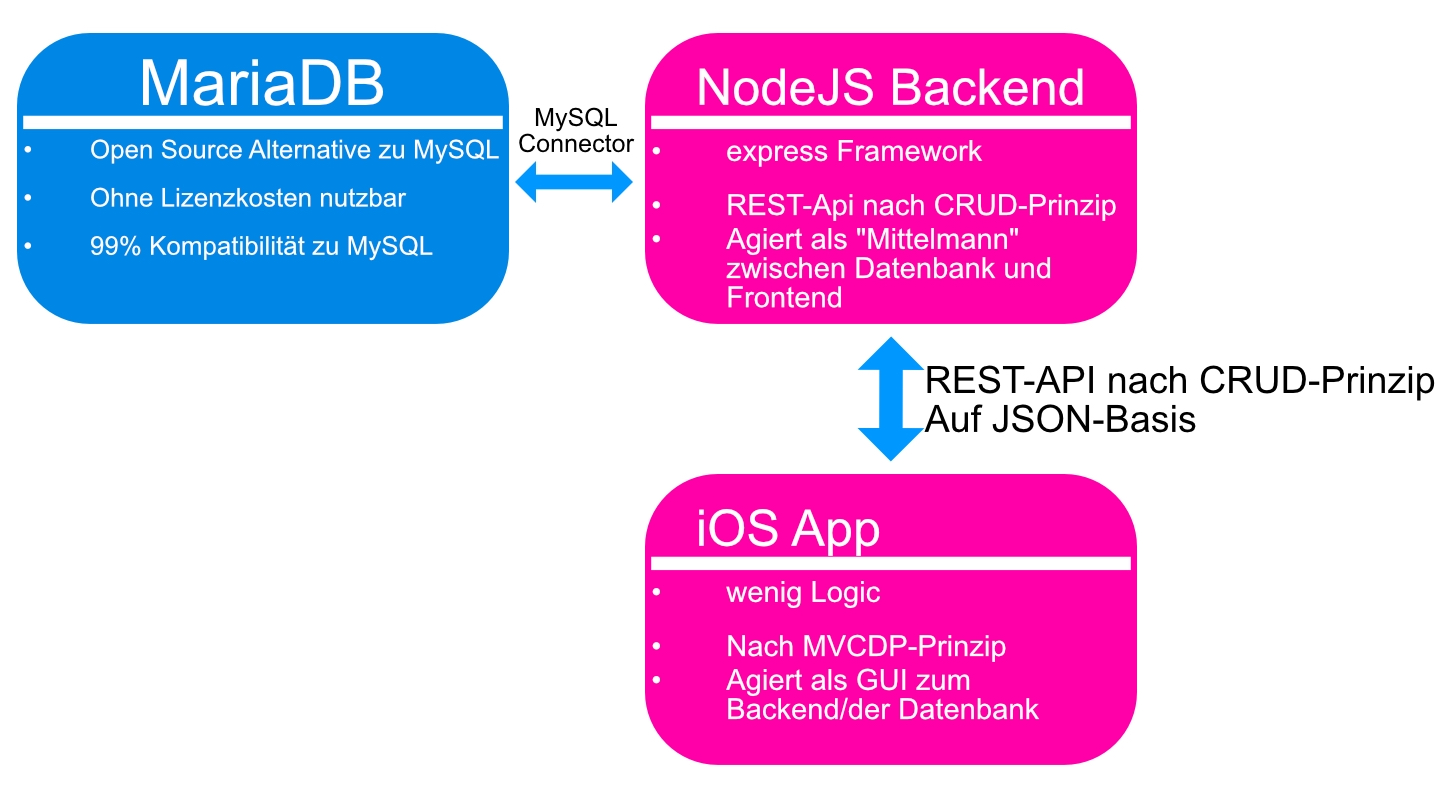
\includegraphics[width=\textwidth]{presentation/image01}
\end{frame}

\section{ER-Diagramm}
\begin{frame}
	\frametitle{ER-Diagramm}
	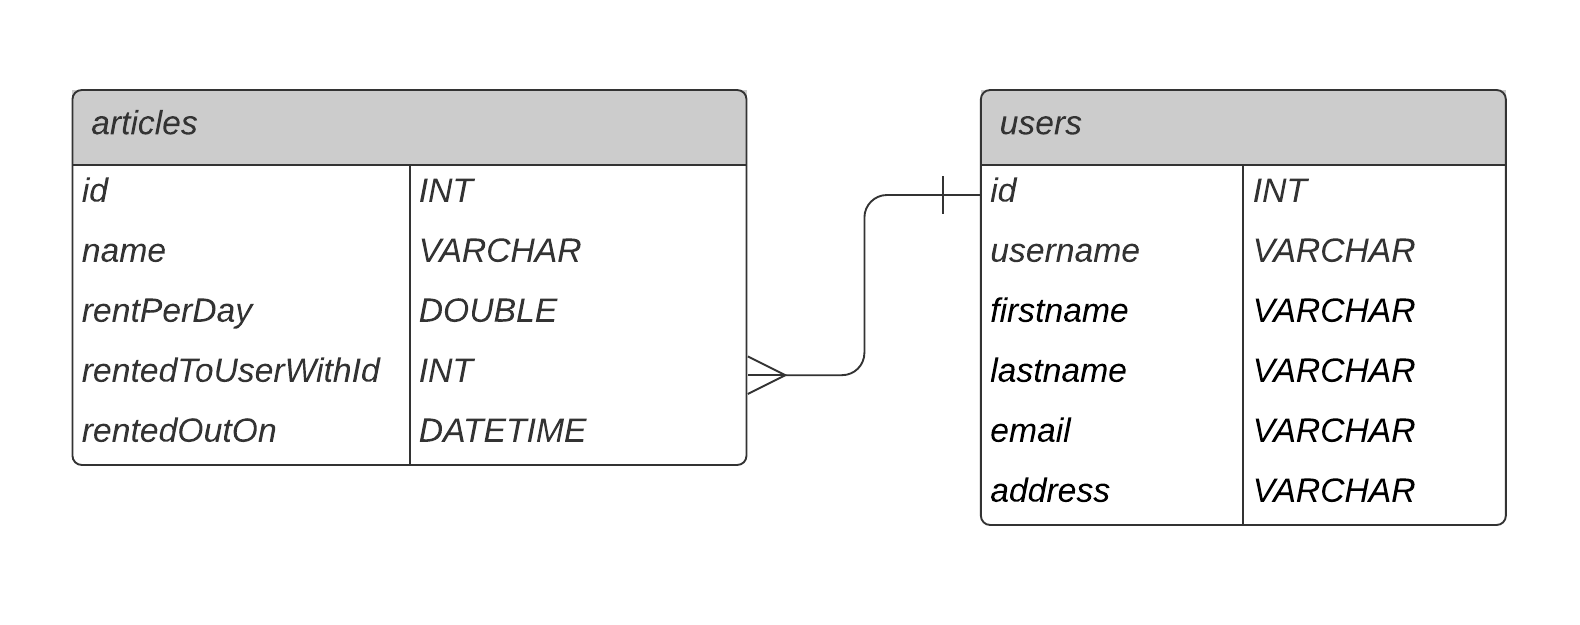
\includegraphics[width=\textwidth]{presentation/image06}
\end{frame}

\section{Implementierung des ER-Diagrams}
\begin{frame}
	\frametitle{Implementierung des ER-Diagrams}
	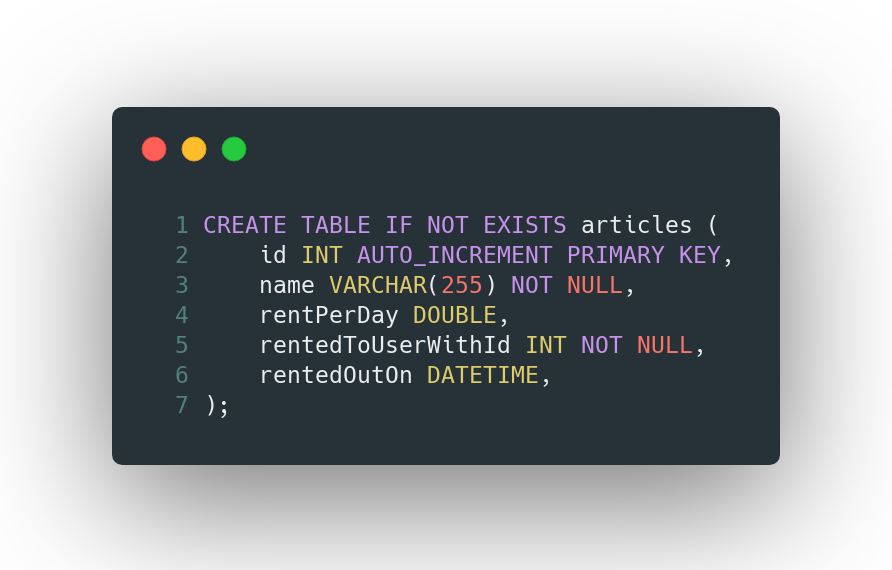
\includegraphics[width=\textwidth]{presentation/image07}
\end{frame}

\begin{frame}
	\frametitle{Implementierung des ER-Diagrams}
	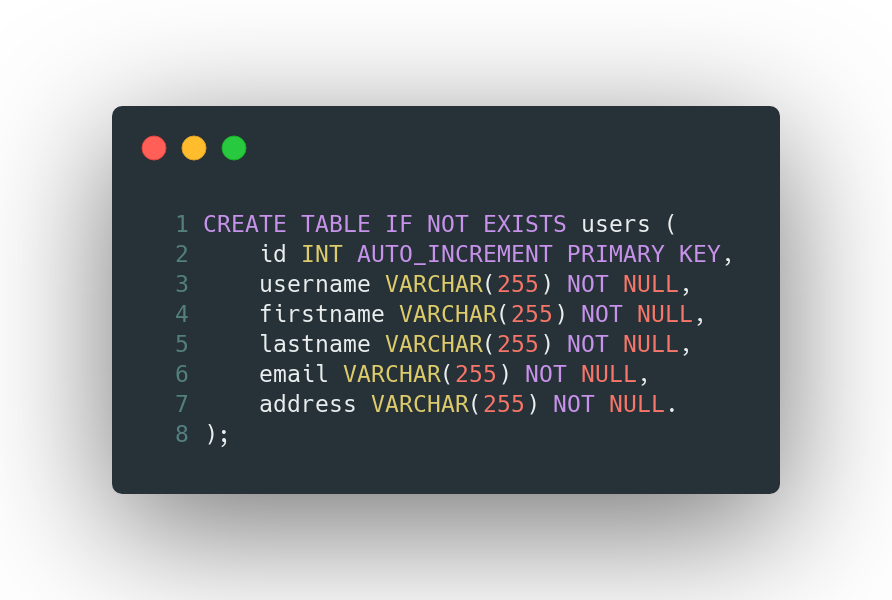
\includegraphics[width=\textwidth]{presentation/image08}
\end{frame}

\section{GUI}
\subsection{Benutzung der Datenbank mithilfe des Backends}
\begin{frame}
	\frametitle{Benutzung der Datenbank mithilfe des Backends - API-Routen}
	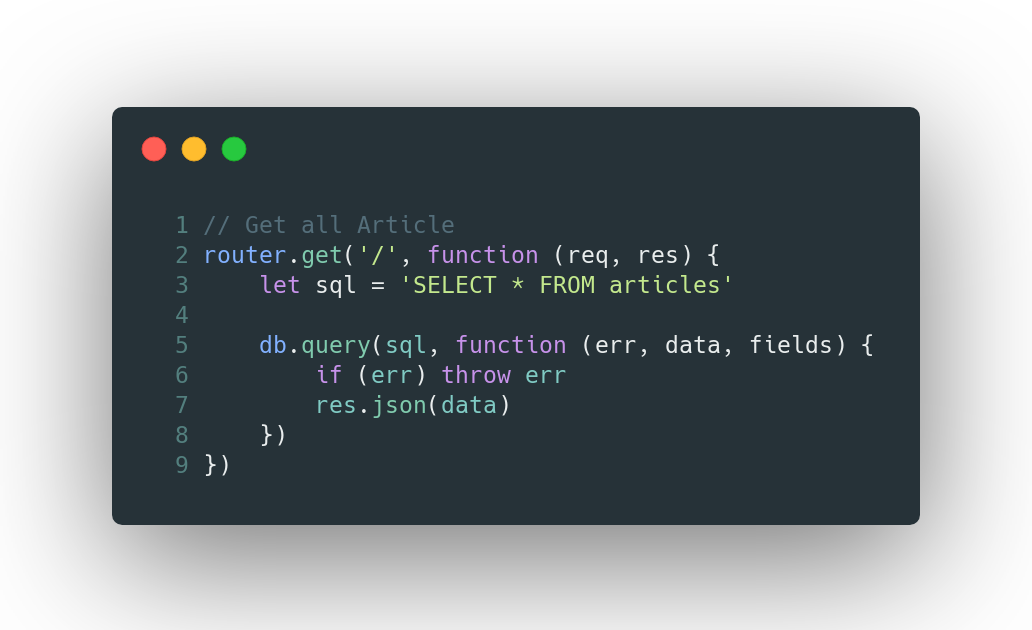
\includegraphics[width=\textwidth]{presentation/image02}
\end{frame}

\begin{frame}
	\frametitle{Benutzung der Datenbank mithilfe des Backends - API-Daten}
	\center
	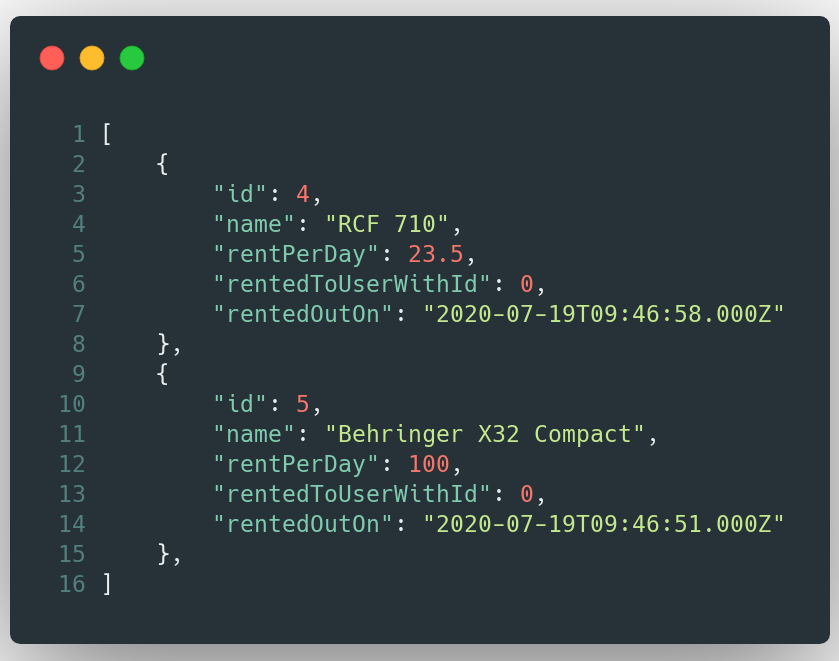
\includegraphics[width=0.8\textwidth]{presentation/image05}
\end{frame}

\begin{frame}
	\frametitle{Benutzung der Datenbank mithilfe des Backends - API-Routen}
	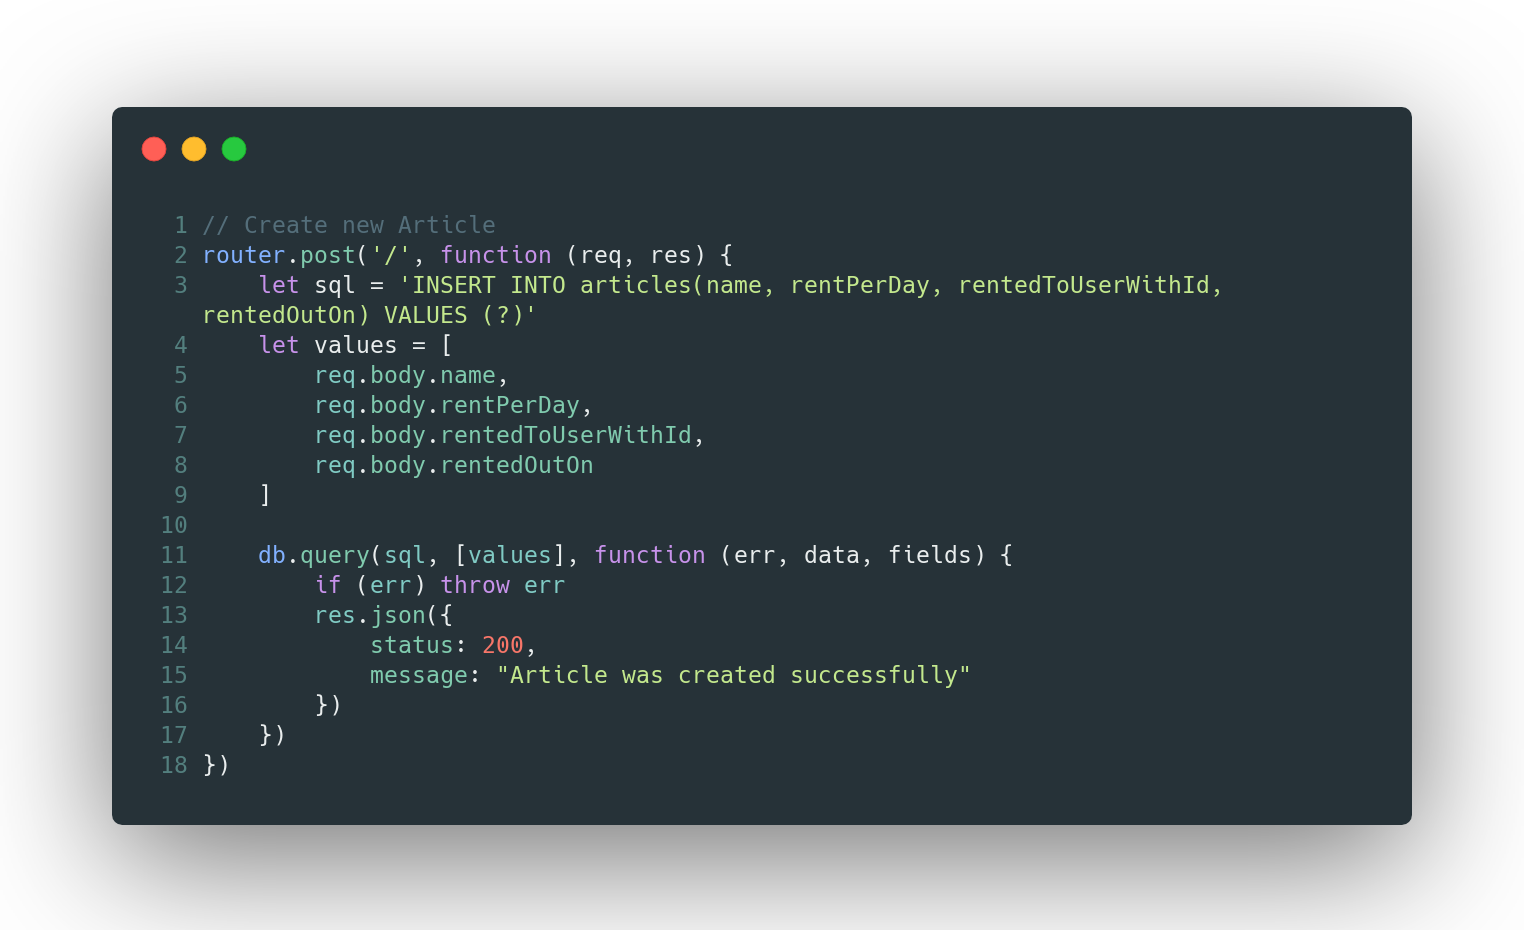
\includegraphics[width=\textwidth]{presentation/image03}
\end{frame}

\begin{frame}
	\frametitle{Benutzung der Datenbank mithilfe des Backends - API-Routen}
	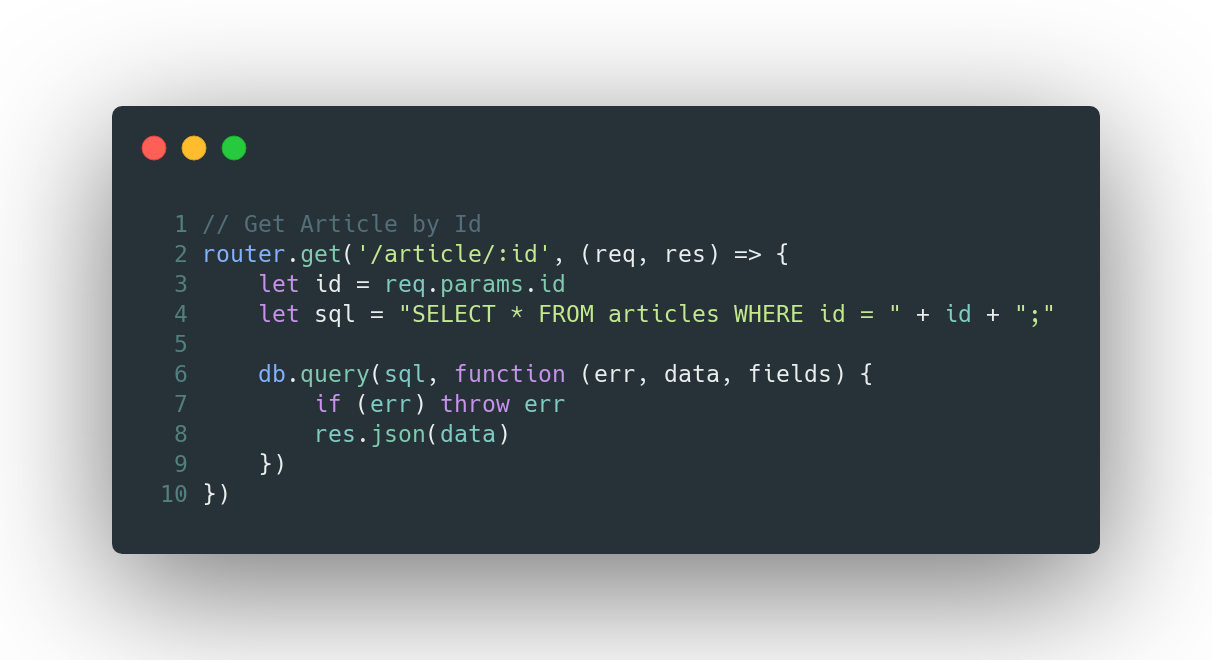
\includegraphics[width=\textwidth]{presentation/image04}
\end{frame}

\subsection{Implementierung des DataProviders}
\begin{frame}
	\frametitle{Implementierung des DataProviders}
	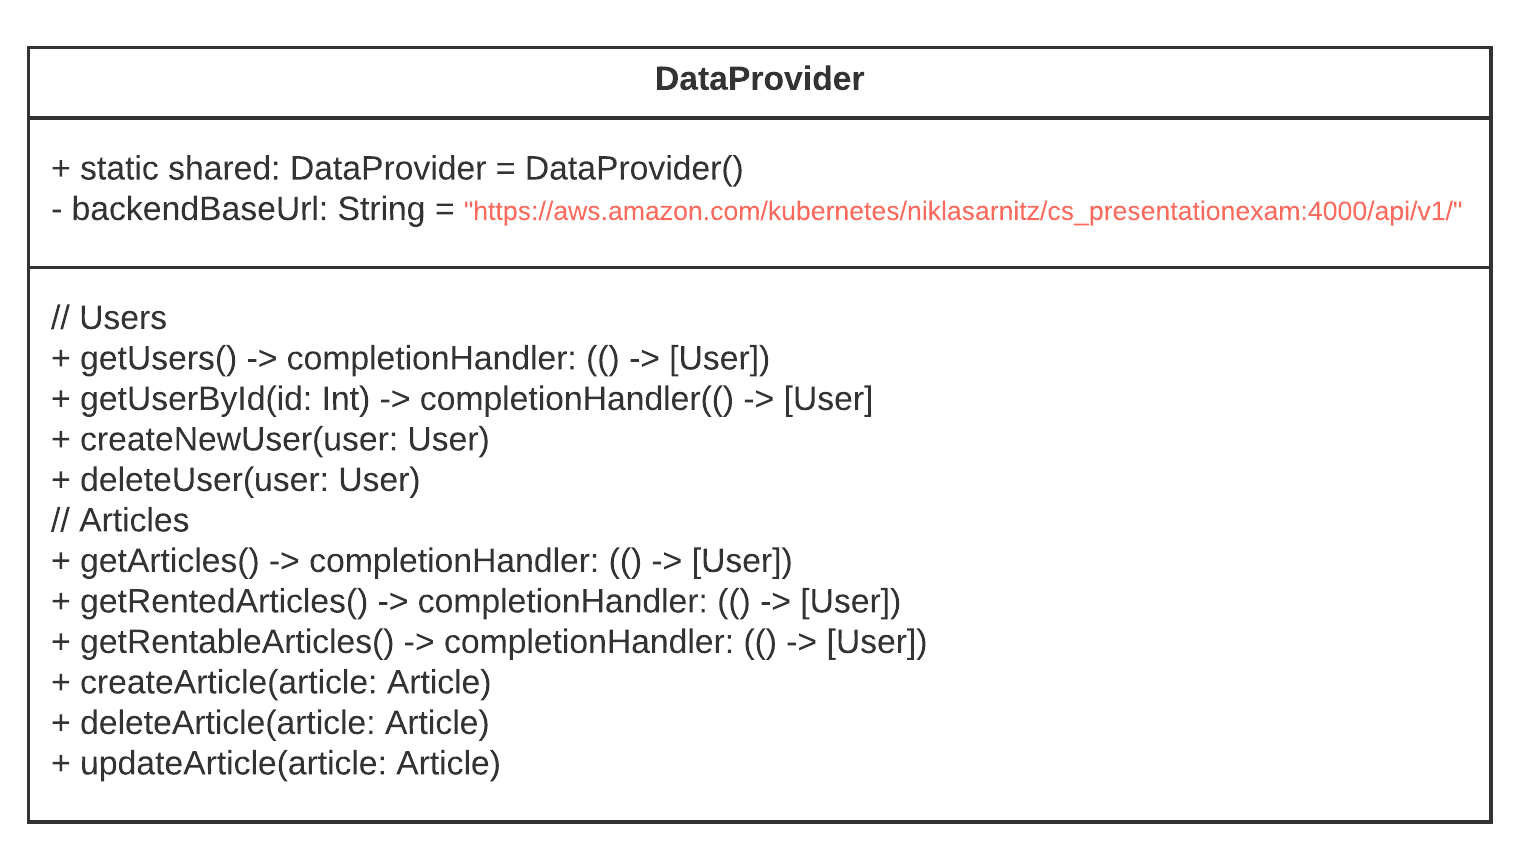
\includegraphics[width=\textwidth]{presentation/image09}
\end{frame}

\subsection{Demo}
\begin{frame}
	\frametitle{Demo}
	\center
	\includemedia[height=0.8\textheight,activate=pageopen,passcontext,transparent,addresource=presentation/demo01.mp4,flashvars={source=presentation/demo01.mp4}]{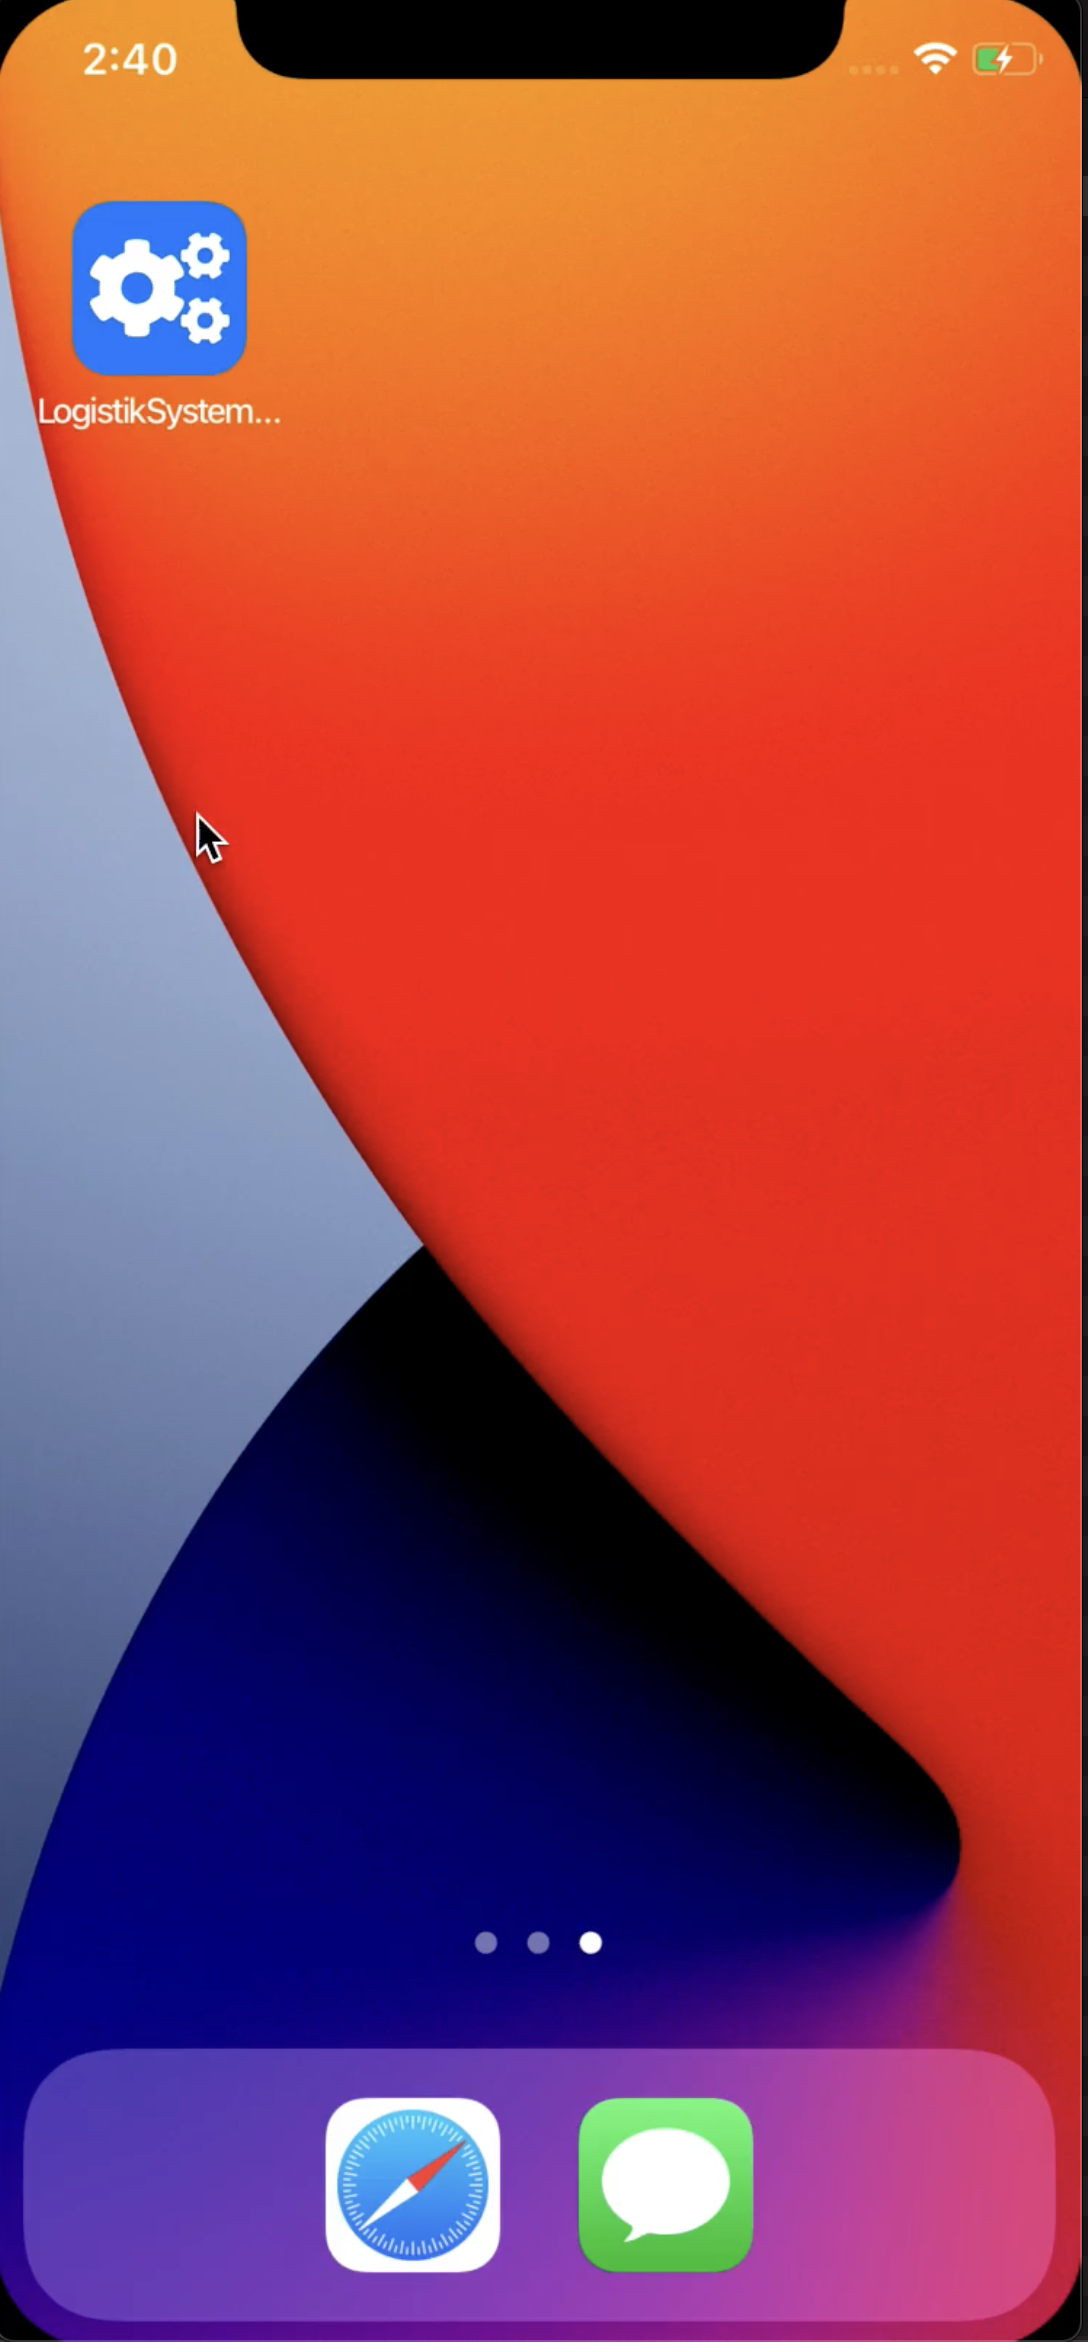
\includegraphics[width=0.6\linewidth]{presentation/demo01}}{presentation/demo01.png}
\end{frame}

\section{Quellen}
\begin{frame}
	\frametitle{Quellen}
	\begin{itemize}
		\item https://dev.mysql.com/doc/ (Stand: 01.07.2020)
		\item https://developer.apple.com/documentation/ (Stand: 01.07.2020)
		\item https://expressjs.com/en/4x/api.html (Stand: 01.07.2020)
	\end{itemize}	
\end{frame}

\begin{frame}
	\center
	\huge{Noch Fragen?}
	Anmerkung: Den code dieses Projekts finden sie unter https://github.com/niklasarnitz/cs-presentation-exam
\end{frame}

\end{document}
